\section{Giao diện Wizard \& Trải nghiệm Người dùng}\label{sec:wizard-interface}

\noindent
Nền Tảng Máy học Toàn Diện sử dụng kiến trúc giao diện wizard tinh vi để mang lại trải nghiệm người dùng liền mạch cho các quy trình làm việc ML phức tức tạp. Thiết kế này tích hợp quản lý phiên làm việc tiên tiến, xử lý lỗi toàn diện và các nguyên tắc thiết kế responsive để tạo ra tương tác trực quan cho người dùng với các mức độ chuyên môn ML khác nhau.

\paragraph{Kiến trúc Technical Implementation:}
AIO Classifier được xây dựng trên Streamlit với implementation thực tế bao gồm SessionManager quản lý session data với wizard\_ui.session\_manager, StreamlitTrainingPipeline cho model training, Cache System sử dụng \texttt{@st.cache\_resource} cho session preference, wizard 5 bước từ \texttt{templates\_wireframe()} đến \texttt{render\_step5\_wireframe()}, Model Factory import từ models.model\_factory cho 13 thuật toán ML, và các Streamlit components với real-time updates. Hệ thống được thử nghiệm trên 2 bộ dữ liệu khác nhau với tổng cộng 78 cấu hình mô hình (39 cho mỗi dataset), đạt được hiệu suất xuất sắc với nhiều mô hình đạt độ chính xác 100\% trên tập kiểm tra.

\subsection{Thiết kế Quy trình 5 Bước}\label{subsec:wizard-overview}

\subsubsection{Tổng quan Luồng Công việc}

AIO Classifier triển khai wizard có cấu trúc 5 bước để hướng dẫn người dùng qua quy trình ML:

\textbf{Luồng 5 Bước của Wizard:}
\begin{enumerate}[leftmargin=*]
    \item \textbf{Dataset Selection \& Upload}: Upload file CSV/Excel với validation tự động, preview tương tác dataset với phát hiện kiểu dữ liệu thông minh, cấu hình sampling với cân bằng categories, kiểm tra chất lượng dữ liệu với phát hiện missing values.
    
    \item \textbf{Data Processing \& Preprocessing}: Chọn cột input và label với validation tự động, cấu hình phân chia train/validation/test dataset, lựa chọn scaler (StandardScaler, MinMaxScaler, RobustScaler), xử lý dữ liệu thiếu và outlier với các chiến lược thông minh.
    
    \item \textbf{Optuna Optimization \& Ensemble Configuration}: Lựa chọn mô hình ML với hỗ trợ 13 thuật toán, cấu hình Optuna cho hyperparameter optimization, thiết kế Voting Ensemble với trọng số tùy chỉnh, cấu hình Stacking Ensemble với meta-learner.
    
    \item \textbf{Training Execution and Monitoring}: Theo dõi tiến trình huấn luyện real-time với progress bars, giám sát hiệu suất và metrics trong quá trình training, cache management thông minh cho tối ưu hóa tốc độ, cấu hình ensemble và tham số chi tiết.
    
    \item \textbf{SHAP Visualization \& Confusion Matrix}: Phân tích SHAP toàn diện với multiple plot types, confusion matrices chi tiết cho từng mô hình, so sánh hiệu suất mô hình với metrics comprehensive, export kết quả multiple formats (CSV, JSON, PNG), báo cáo tổng hợp với visualizations professional.
\end{enumerate}

\begin{figure}[H]
    \centering
\begin{tikzpicture}[scale=0.65]
% Define colors
\definecolor{darkgreen}{RGB}{34,139,34}
\definecolor{darkorange}{RGB}{255,140,0}
\definecolor{orange}{RGB}{255,165,0}

% Define styles with better spacing
\tikzset{
    step1/.style={rectangle, rounded corners, minimum width=2.2cm, minimum height=0.9cm, text width=2cm, text centered, draw=darkgreen, fill=darkgreen!15, font=\small},
    stepc/.style={rectangle, rounded corners, minimum width=2.2cm, minimum height=0.9cm, text width=2cm, text centered, draw=darkorange, fill=darkorange!15, font=\small},
    step5/.style={rectangle, rounded corners, minimum width=2.2cm, minimum height=0.9cm, text width=2cm, text centered, draw=orange, fill=orange!15, font=\small},
    arrow/.style={thick,->,>=stealth}
}

% Step nodes with maximum spacing
\node (step1) [step1] at (0,0) {Bước 1 Lựa chọn Dataset};
\node (step2) [stepc] at (4,0) {Bước 2 Tiền xử lý};
\node (step3) [stepc] at (8,0) {Bước 3 Cấu hình Mô hình};
\node (step4) [stepc] at (12,0) {Bước 4 Huấn luyện};
\node (step5) [step5] at (16,0) {Bước 5 Trực quan hóa};

% Arrows with colors
\draw [arrow, darkgreen] (step1) -- (step2);
\draw [arrow, darkorange] (step2) -- (step3);
\draw [arrow, darkorange] (step3) -- (step4);
\draw [arrow, orange] (step4) -- (step5);

% Labels below steps with maximum spacing
\node [text width=3.5cm, align=center, font=\tiny, text=darkgreen] at (0,-2) {
    Upload files\\
    Data preview\\
    Sampling config
};

\node [text width=3.5cm, align=center, font=\tiny, text=darkorange] at (4,-2) {
    Phát hiện đặc trưng\\
    Tùy chọn phân chia\\
    Validation rules
};

\node [text width=3.5cm, align=center, font=\tiny, text=darkorange] at (8,-2) {
    Lựa chọn mô hình\\
    Tham số Optuna\\
    Ensemble config
};

\node [text width=3.5cm, align=center, font=\tiny, text=darkorange] at (12,-2) {
    Tiến trình huấn luyện\\
    Metrics theo thời gian thực\\
    Quản lý cache
};

\node [text width=3.5cm, align=center, font=\tiny, text=orange] at (16,-2) {
    SHAP analysis\\
    Confusion matrices\\
    Results export
};
\end{tikzpicture}
\caption{Quy trình Wizard 5 Bước của AIO Classifier}
\label{fig:wizard_workflow}
\end{figure}

\textbf{Bước 1 - Lựa chọn Bộ dữ liệu và Cấu hình}:

\begin{figure}[H]
    \centering
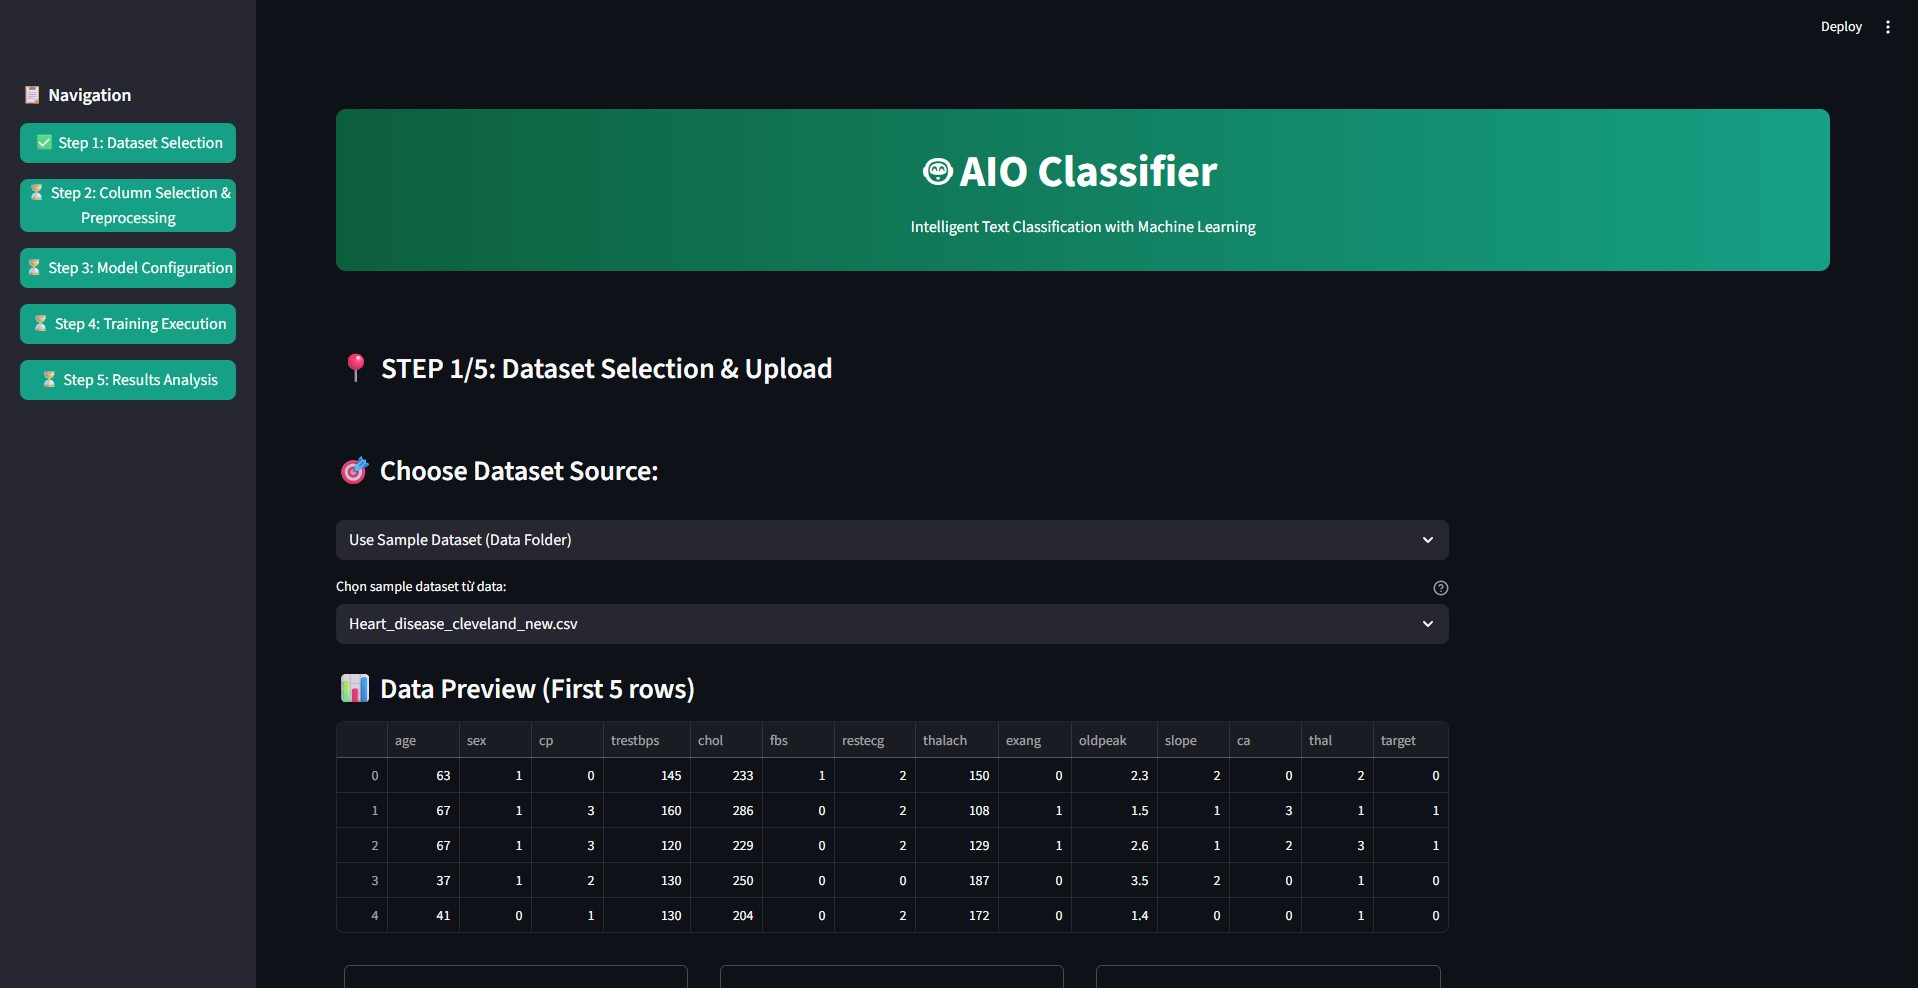
\includegraphics[width=\textwidth]{UI/Step 1.jpg}
\caption{Giao diện Step 1: Dataset Selection và Upload - Tải file và preview dữ liệu}
\label{fig:wizard_step1_real}
\end{figure}

\begin{itemize}
    \item \textbf{Thành phần Tải tệp}: \texttt{st.file\_uploader} với validation cho CSV/Excel files
    \item \textbf{Xem trước Bộ dữ liệu}: \texttt{st.dataframe} preview với automatic column type detection
    \item \textbf{Cấu hình Phân mẫu}: Sampling options với category balancing capabilities
    \item \textbf{Kiểm tra Chất lượng Dữ liệu}: Automatic missing value detection và data quality checks
\end{itemize}

\textbf{Bước 2 - Pipeline Tiền xử lý}:

\begin{figure}[H]
    \centering
\subfloat[Phần 1: Column Selection và Configuration]{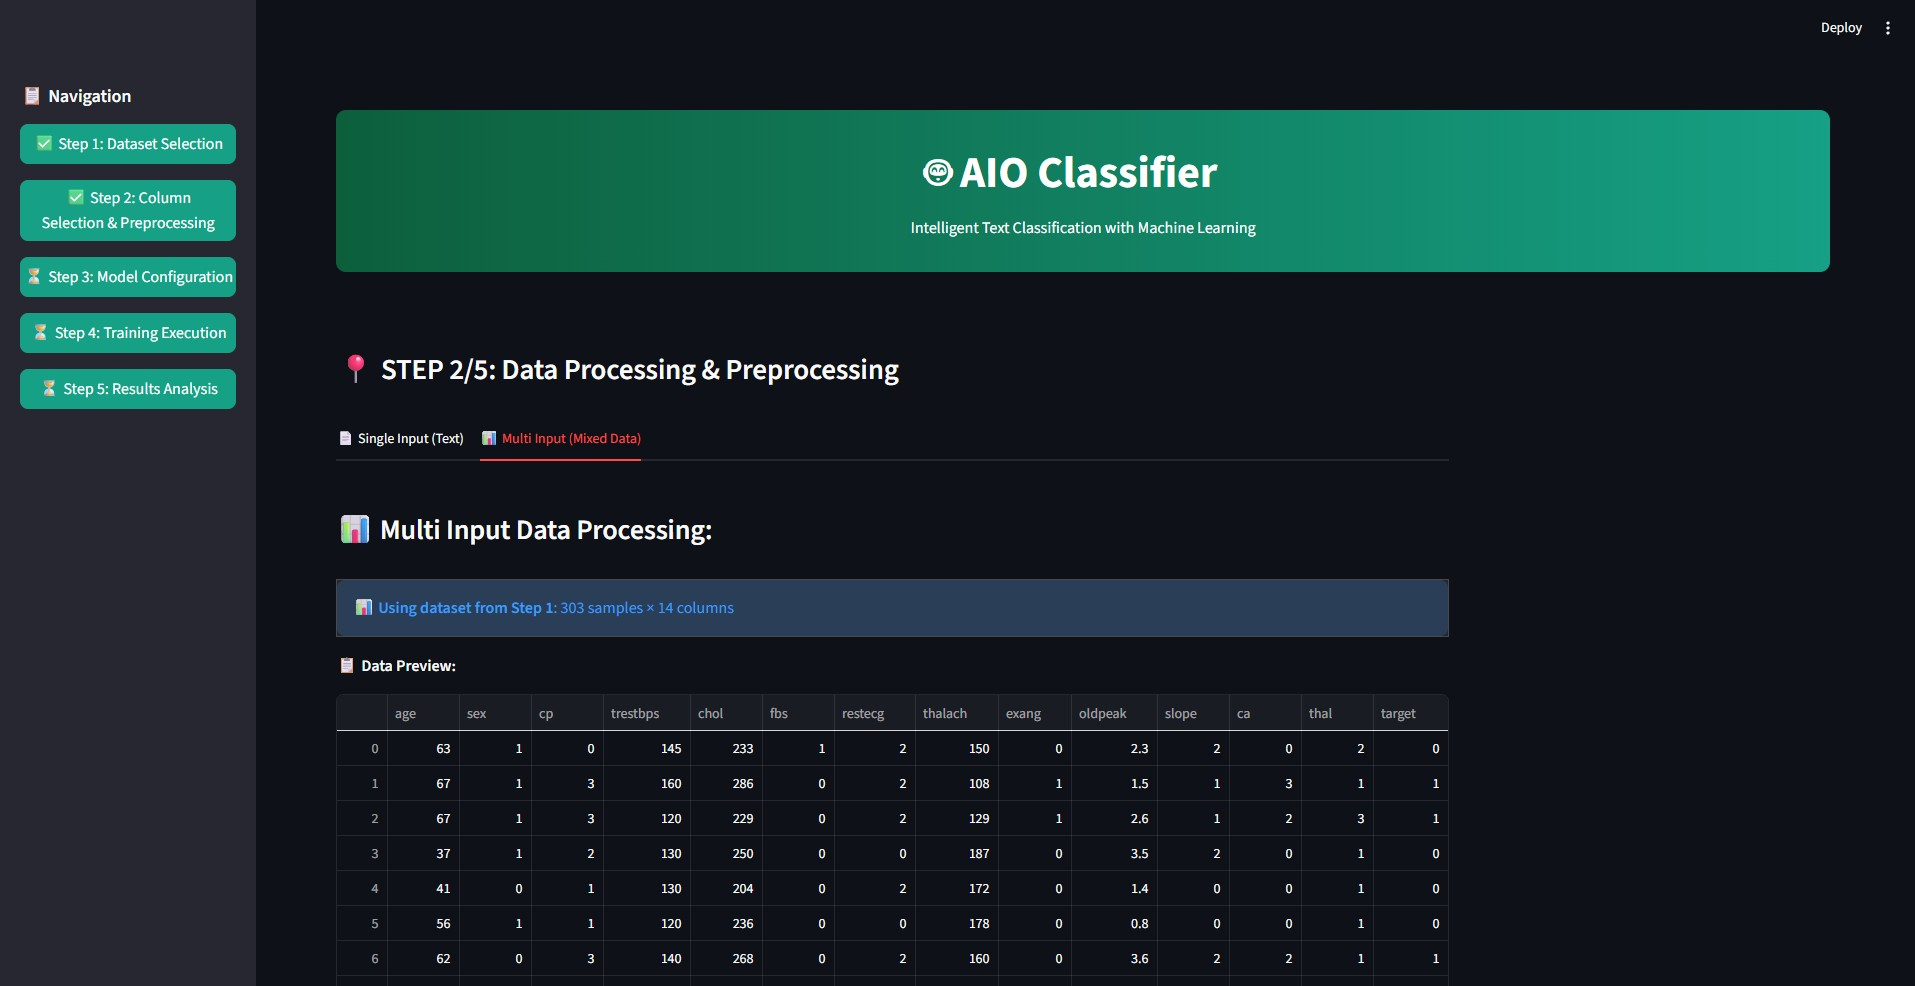
\includegraphics[width=0.48\textwidth]{UI/Step2-1.jpg}}
\quad
\subfloat[Phần 2: Data Processing và Sampling]{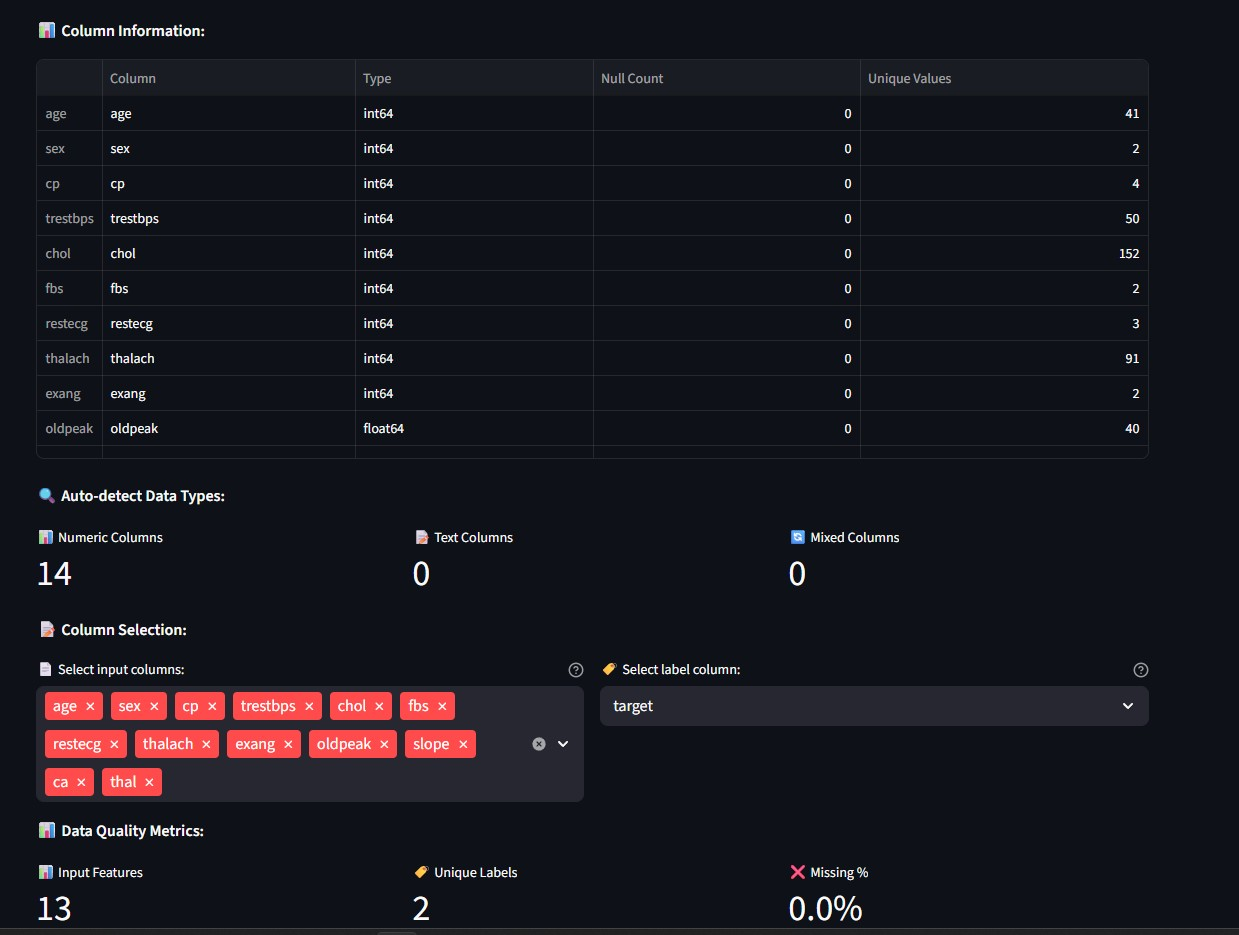
\includegraphics[width=0.48\textwidth]{UI/Step2-2.jpg}}
\caption{Giao diện Step 2: Data Processing và Preprocessing với 2 phần}
\label{fig:wizard_step2_real}
\end{figure}

\begin{itemize}
    \item \textbf{Column Selection}: st.selectbox để chọn input và label columns
    \item \textbf{Tùy chọn Scaling}: Streamlit selectors cho StandardScaler, MinMaxScaler, RobustScaler
    \item \textbf{Data Splitting}: Train/validation/test split configuration với custom ratios
    \item \textbf{Missing Data Handling}: Automatic handling strategies cho missing values
\end{itemize}

\textbf{Bước 3 - Cấu hình Mô hình}:

\begin{figure}[H]
    \centering
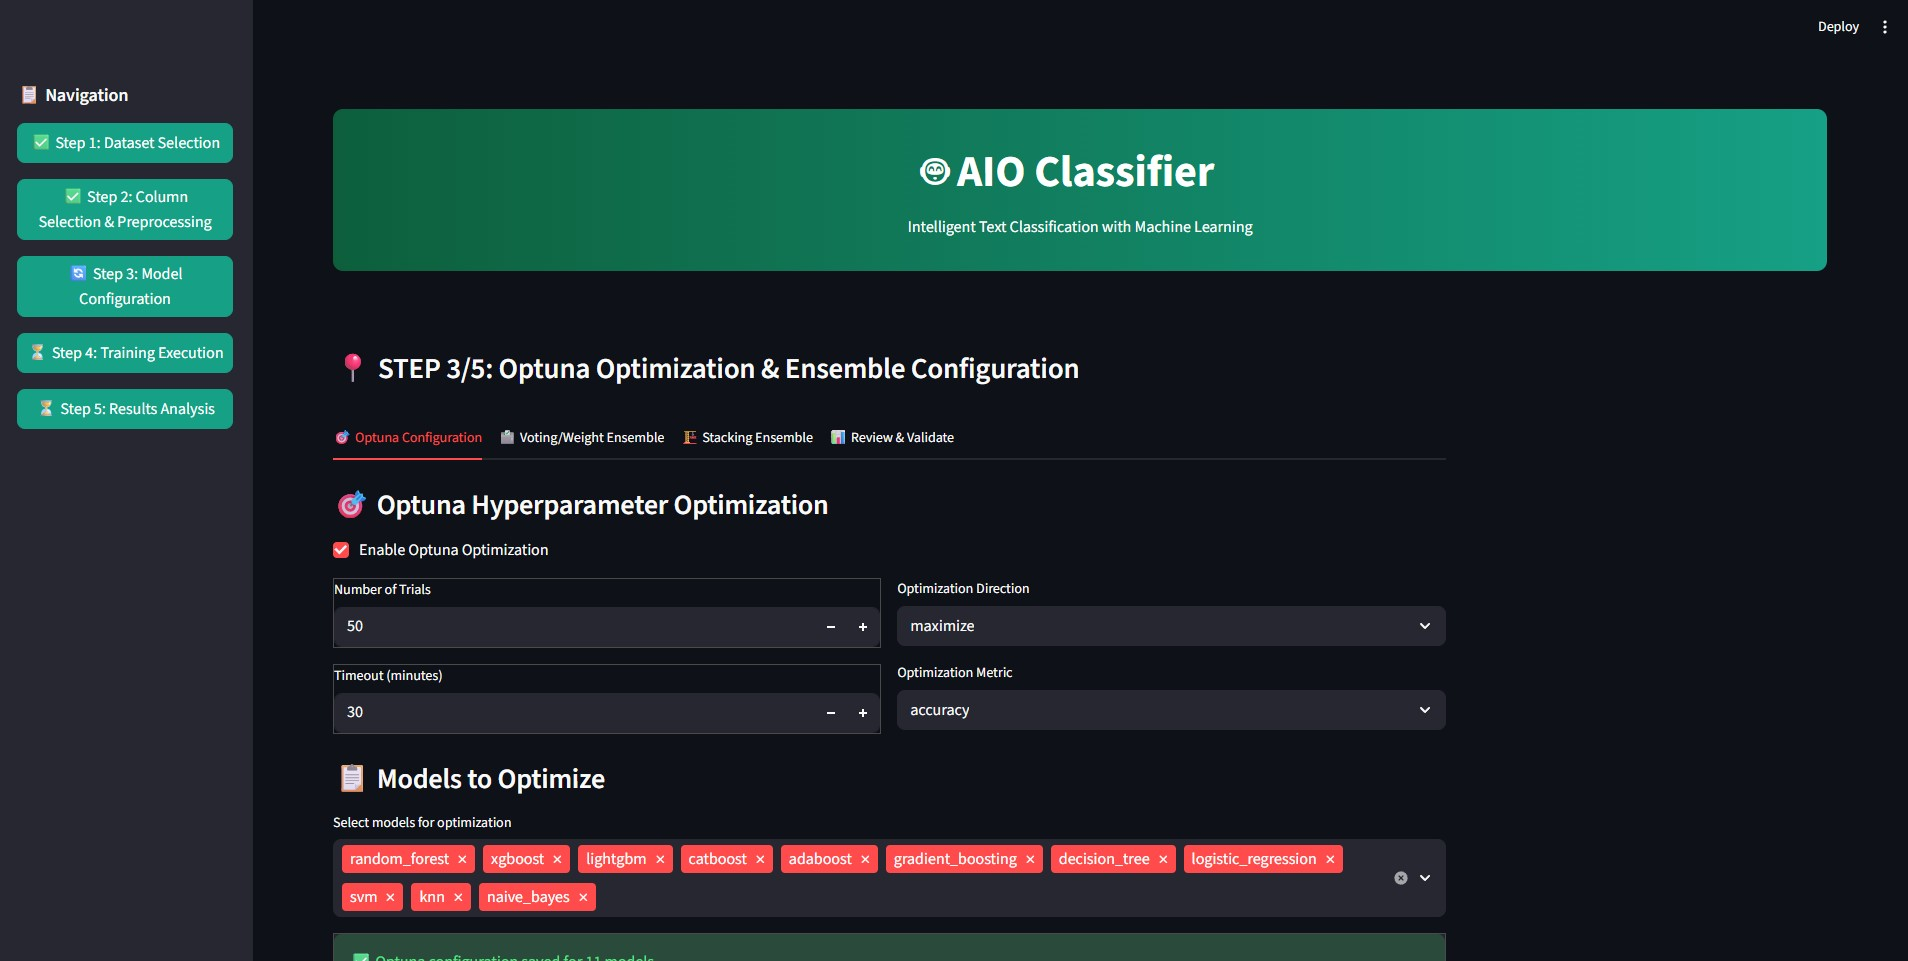
\includegraphics[width=\textwidth]{UI/Step 3.jpg}
\caption{Giao diện Step 3: Optuna Optimization và Ensemble Configuration}
\label{fig:wizard_step3_real}
\end{figure}

\begin{itemize}
    \item \textbf{Model Selection}: st.multiselect cho chọn multiple ML models từ 13 algorithms
    \item \textbf{Optuna Configuration}: Hyperparameter optimization settings với trial numbers
    \item \textbf{Voting Ensemble}: Configuration cho voting với custom weights
    \item \textbf{Stacking Ensemble}: Configuration cho stacking với meta-learner selection
\end{itemize}

\textbf{Bước 4 - Thực thi Huấn luyện}:

\begin{figure}[H]
    \centering
\subfloat[Training Progress và Monitoring]{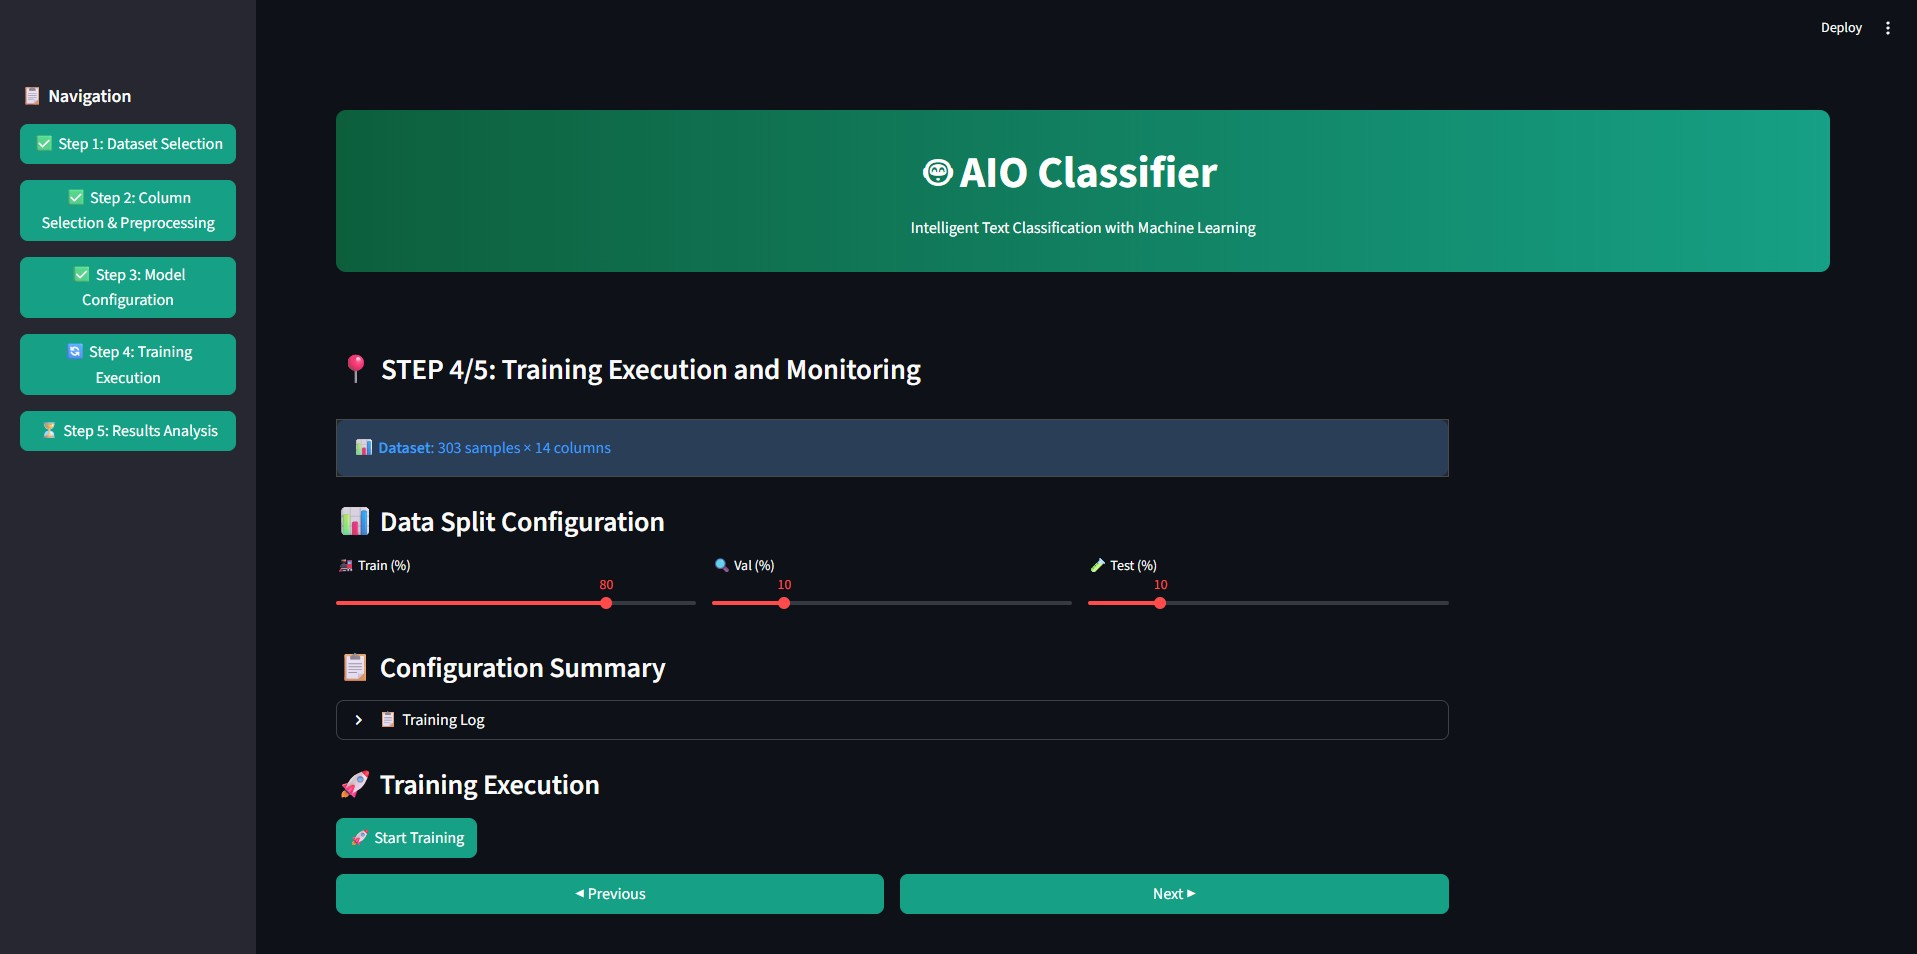
\includegraphics[width=0.48\textwidth]{UI/Step 4.jpg}}
\quad
\subfloat[Advanced Training Configuration]{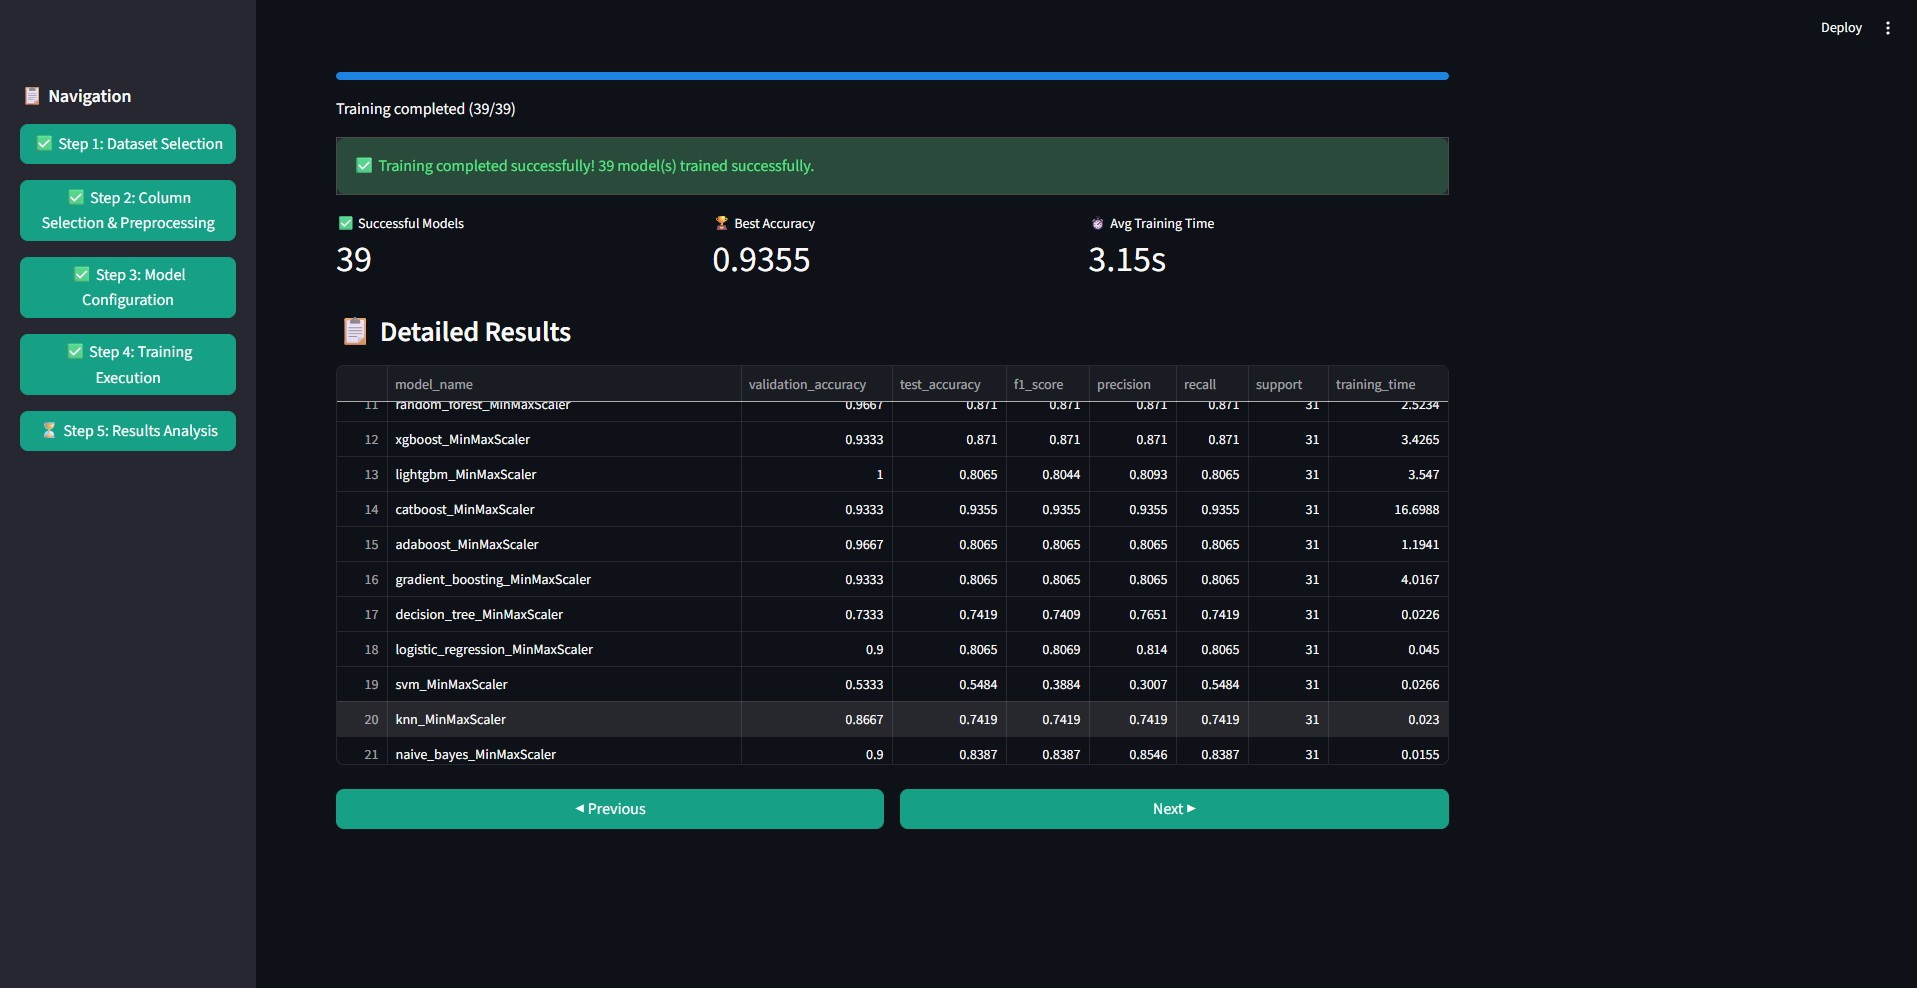
\includegraphics[width=0.48\textwidth]{UI/Step 4 -2.jpg}}
\caption{Giao diện Step 4: Training Execution and Monitoring với 2 phần}
\label{fig:wizard_step4_real}
\end{figure}

\begin{itemize}
    \item \textbf{Training Progress}: \texttt{st.progress\_bar} và status text cho real-time monitoring
    \item \textbf{Performance Metrics}: Live accuracy và loss metrics during training
    \item \textbf{Cache Management}: Intelligent caching của model results và predictions
    \item \textbf{Ensemble Training}: Batch training với multiple models và ensemble methods
\end{itemize}

\textbf{Bước 5 - Trực quan hóa \& Phân tích}:

\begin{figure}[H]
\centering
\subfloat[Main Results Interface]{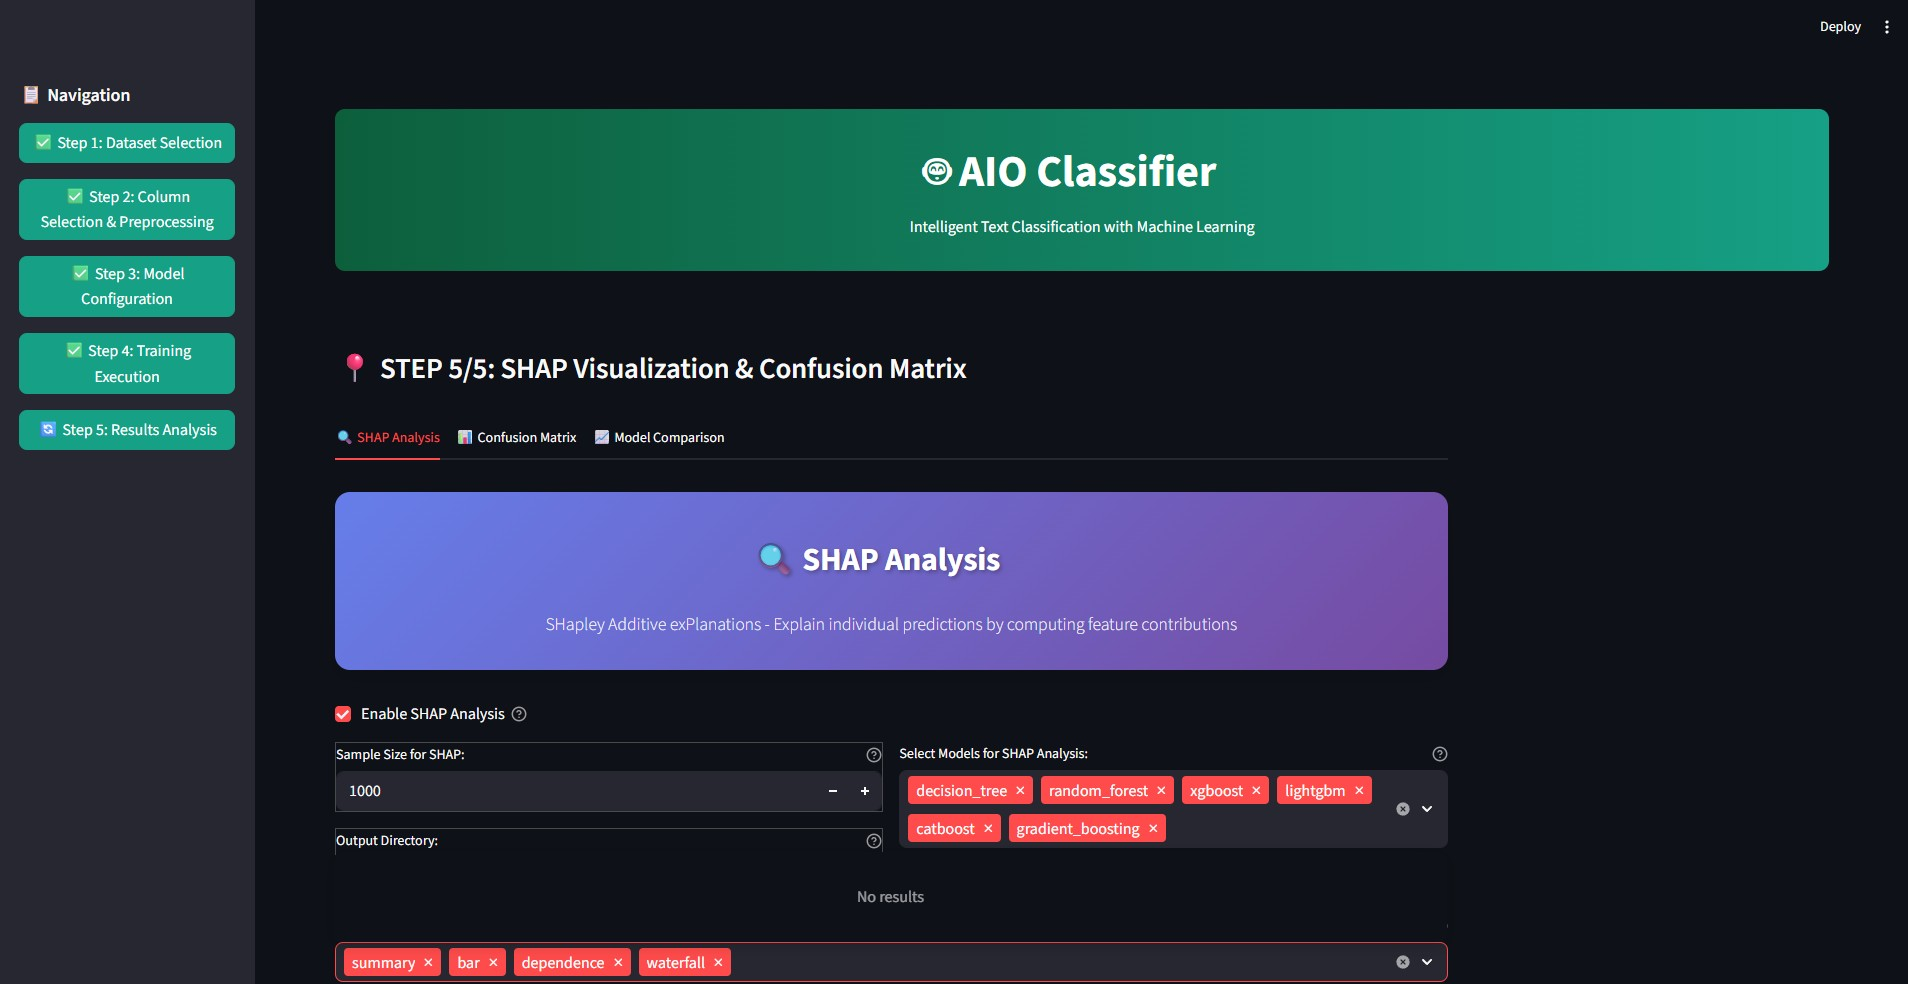
\includegraphics[width=0.48\textwidth]{UI/Step5-1.jpg}}
\quad
\subfloat[SHAP Analysis Visualization]{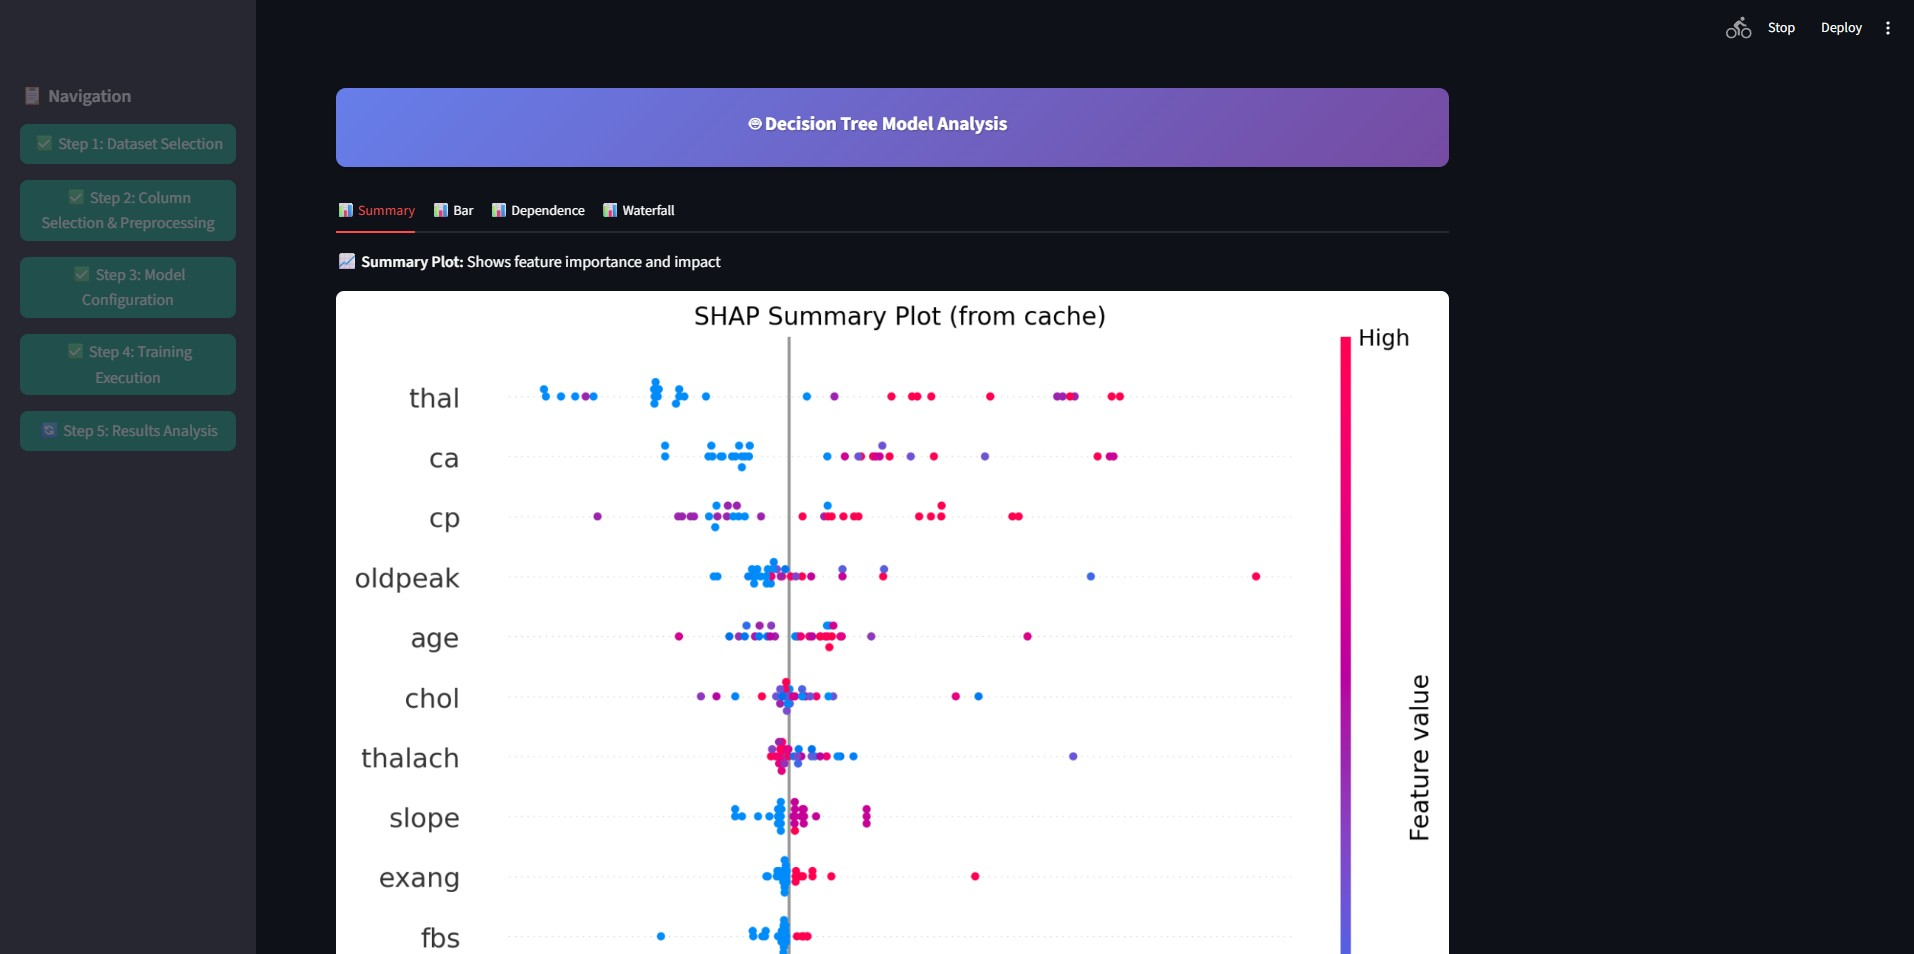
\includegraphics[width=0.48\textwidth]{UI/Step5-2.jpg}}
\caption{Giao diện Step 5: SHAP Visualization và Confusion Matrix Analysis}
\label{fig:wizard_step5_real_1_2}
\end{figure}

\begin{figure}[H]
    \centering
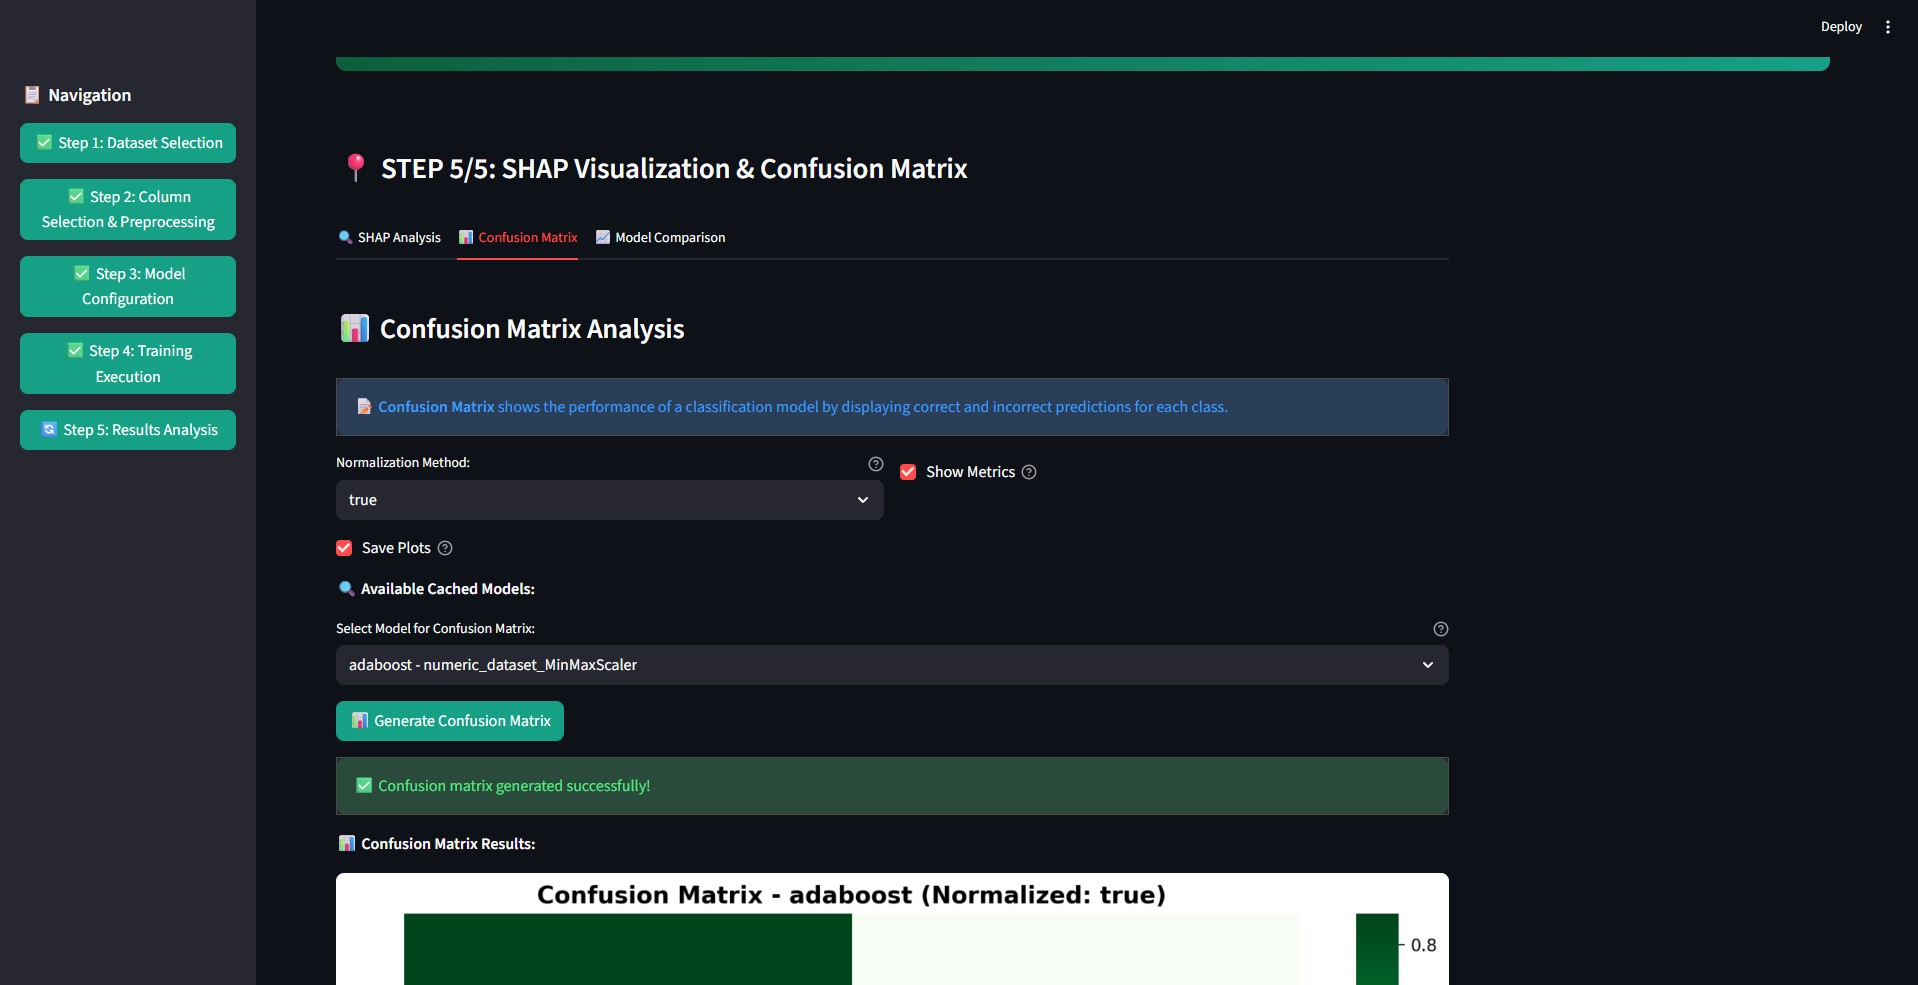
\includegraphics[width=\textwidth]{UI/Step5-3.jpg}
\caption{Giao diện Step 5: AIO Classifier Model Comparison và Export}
\label{fig:wizard_step5_real_3}
\end{figure}

\begin{itemize}
    \item \textbf{SHAP Analysis}: Multiple SHAP plot types với feature importance
    \item \textbf{Confusion Matrices}: Detailed visualization cho từng model performance
    \item \textbf{Model Comparison}: AIO Classifier metrics comparison across models
    \item \textbf{Export Capabilities}: Multiple formats (CSV, PNG, JSON) với custom naming
\end{itemize}

\subsection{Session Management System}\label{subsec:session-management}

\subsubsection{Quản lý Trạng thái Phiên Tiên tiến}

\textbf{Kiến trúc Trạng thái Phiên}:
\begin{itemize}
    \item \textbf{Duy trì Trạng thái}: Trạng thái phiên toàn diện với tự động lưu và các cơ chế sao lưu
    \item \textbf{Theo dõi Tiến trình}: Theo dõi tiến trình chi tiết qua tất cả các bước wizard với khả năng làm tiếp
    \item \textbf{Quản lý Cấu hình}: Lưu trữ tập trung các cấu hình và tùy chọn của người dùng
    \item \textbf{Tích hợp Cache}: Cache nhận biết phiên để tối ưu hóa hiệu suất và giảm dư thừa
\end{itemize}

\textbf{Cơ chế Phục hồi Phiên}:
\begin{itemize}
    \item \textbf{Tự động Lưu}: Lưu tự động trạng thái phiên sau mỗi hành động quan trọng
    \item \textbf{Hệ thống Sao lưu}: Sao lưu định kỳ để bảo vệ tiến trình người dùng
    \item \textbf{Tùy chọn Phục hồi}: Phục hồi mượt mà từ sự cố hệ thống hoặc gián đoạn mạng
    \item \textbf{Định giá Dữ liệu}: Định giá dữ liệu phiên được phục hồi để đảm bảo tính toàn vẹn
\end{itemize}

\begin{figure}[H]
    \centering
\begin{tikzpicture}[node distance=1.2cm]
% Define colors
\definecolor{darkgreen}{RGB}{34,139,34}
\definecolor{darkorange}{RGB}{255,140,0}
\definecolor{orange}{RGB}{255,165,0}

% Define styles for flow diagram
\tikzset{
    process/.style={rectangle, minimum width=3cm, minimum height=0.8cm, text centered, draw=darkorange, fill=darkorange!15},
    decision/.style={diamond, minimum width=2cm, minimum height=1cm, text centered, draw=orange, fill=orange!15},
    data/.style={cylinder, minimum width=2cm, minimum height=1cm, text centered, draw=darkgreen, fill=darkgreen!15},
    arrow/.style={thick,->,>=stealth}
}

% Process nodes
\node (start) [process] {User Action};
\node (validate) [decision, below=of start] {Validation Required?};
\node (process) [process, below=of validate] {Process Action};
\node (save) [process, below=of process] {Auto-Save Session};
\node (update) [data, below=of save] {Update Session State};
\node (backup) [process, left=of update, xshift=-2cm] {Periodic Backup};
\node (recovery) [process, right=of update, xshift=2cm] {Recovery Check};

% Arrows with colors
\draw [arrow, darkorange] (start) -- (validate);
\draw [arrow, orange] (validate) -- node[right, font=\tiny] {Có} (process);
\draw [arrow, darkorange] (validate.west) -- node[above, font=\tiny] {Không} (process.west);
\draw [arrow, darkorange] (process) -- (save);
\draw [arrow, darkgreen] (save) -- (update);
\draw [arrow, darkorange] (update) -- (backup);
\draw [arrow, darkorange] (update) -- (recovery);

% Additional flow indicators
\draw [arrow, dashed, darkgreen] (backup) -- node[above, font=\tiny] {Every 30s} (update);
\end{tikzpicture}
\caption{Biểu đồ Luồng Quản lý Phiên}
\label{fig:session_management}
\end{figure}

\subsubsection{Streamlit Session Management}

\textbf{Session State Management}:
\begin{itemize}
    \item \textbf{SessionManager}: Sử dụng wizard\_ui.session\_manager cho session persistence
    \item \textbf{Step Data}: Lưu trữ dữ liệu từng bước với \texttt{get\_step\_data()} và \texttt{set\_step\_data()}
    \item \textbf{Navigation}: Điều hướng giữa các bước với \texttt{get\_current\_step()} và \texttt{set\_current\_step()}
    \item \textbf{Cache Resource}: \texttt{@st.cache\_resource} cho session management persistence
\end{itemize}

\textbf{Implementation chi tiết SessionManager}:

\begin{minted}{python}
class SessionManager:
    """Manages Streamlit session state for the wizard interface"""
    
    def __init__(self):
        self.session_key = "wizard_session"
        self.backup_file = "wizard_ui/session_backup.json"
        
    def initialize_session(self):
        """Initialize session with default values"""
        if self.session_key not in st.session_state:
            st.session_state[self.session_key] = {
                'current_step': 1,
                'step_data': {},
                'step_status': {},
                'configuration': {},
                'errors': [],
                'last_updated': datetime.now().isoformat()
            }
            
    def save_step_data(self, step: int, data: Dict[str, Any]):
        """Save data for specific step"""
        session = st.session_state[self.session_key]
        session['step_data'][step] = data
        session['last_updated'] = datetime.now().isoformat()
        
        # Auto-save to backup file
        self.save_to_backup()
        
    def get_step_data(self, step: int) -> Dict[str, Any]:
        """Get data for specific step"""
        session = st.session_state[self.session_key]
        return session['step_data'].get(step, {})
        
    def clear_session(self):
        """Clear all session data"""
        if self.session_key in st.session_state:
            del st.session_state[self.session_key]
        self.initialize_session()
\end{minted}

\textbf{Step Manager và Navigation System}:

\begin{minted}{python}
class StepStatus(Enum):
    """Enumeration for step completion status"""
    PENDING = "pending"
    IN_PROGRESS = "in_progress"
    COMPLETED = "completed"
    BLOCKED = "blocked"
    ERROR = "error"

class StepManager:
    """Manages wizard steps and transitions"""
    
    def __init__(self):
        self.current_step = 1
        self.step_status = {i: StepStatus.PENDING for i in range(1, 6)}
        self.step_data = {}
        
    def get_current_step(self) -> int:
        """Get current active step"""
        return self.current_step
        
    def can_proceed_to_step(self, step: int) -> bool:
        """Check if user can proceed to specified step"""
        # Check if all previous steps are completed
        for i in range(1, step):
            if self.step_status[i] != StepStatus.COMPLETED:
                return False
        return True
        
    def complete_step(self, step: int, data: Dict[str, Any]):
        """Mark step as completed and store data"""
        self.step_status[step] = StepStatus.COMPLETED
        self.step_data[step] = data
\end{minted}

\subsection{Error Handling \& Recovery}\label{subsec:error-handling}

\subsubsection{AIO Classifier Error Management}

\textbf{Hệ thống Phân loại Lỗi}:
\begin{itemize}
    \item \textbf{Lỗi Người dùng}: Lỗi xác thực đầu vào với hướng dẫn sửa lỗi rõ ràng
    \item \textbf{Lỗi Hệ thống}: Lỗi kỹ thuật với các nỗ lực phục hồi tự động
    \item \textbf{Lỗi Dữ liệu}: Vấn đề chất lượng dữ liệu với các gợi ý thông minh để giải quyết
    \item \textbf{Lỗi Tài nguyên}: Vấn đề về bộ nhớ và tài nguyên tính toán với sự suy giảm mượt mà
\end{itemize}

\textbf{Recovery Mechanisms}:
\begin{itemize}
    \item \textbf{Thử lại Tự động}: Logic thử lại thông minh cho các lỗi tạm thời với backoff theo cấp số nhân
    \item \textbf{Suy giảm Mượt mà}: Hệ thống tiếp tục hoạt động với chức năng giảm khi có thể
    \item \textbf{Hướng dẫn Người dùng}: Hướng dẫn rõ ràng cho người dùng để giải quyết các lỗi có thể phục hồi
    \item \textbf{Bảo toàn Ngữ cảnh}: Duy trì ngữ cảnh của người dùng và tiến trình trong quá trình phục hồi lỗi
\end{itemize}

\subsubsection{Khung Định giá}

\textbf{Định giá Theo thời gian thực}:
\begin{itemize}
    \item \textbf{Định giá Đầu vào}: Phản hồi ngay lập tức cho các đầu vào của người dùng với thông báo lỗi rõ ràng
    \item \textbf{Định giá Dữ liệu}: Kiểm tra chất lượng dữ liệu toàn diện với các đề xuất có thể thực hiện
    \item \textbf{Kiểm tra Phụ thuộc}: Đảm bảo các yêu cầu được đáp ứng trước khi cho phép tiến triển
    \item \textbf{Định giá Tài nguyên}: Kiểm tra khả dụng của tài nguyên trước khi khởi tạo các hoạt động
\end{itemize}

\subsection{Kiến trúc Thiết kế Responsive}\label{subsec:responsive-design}

\subsubsection{Các Thành phần Giao diện Thích ứng}

\textbf{Streamlit UI Components}:
\begin{itemize}
    \item \textbf{Wireframe Layout}: Cấu trúc 5-step wizard với render\_step*\_wireframe() functions
    \item \textbf{Interactive Elements}: \texttt{st.selectbox}, \texttt{st.button}, \texttt{st.file\_uploader} cho user interaction
    \item \textbf{Progress Indicators}: Progress bars và status text cho training monitoring
    \item \textbf{Data Display}: \texttt{st.dataframe}, \texttt{st.table} cho dataset preview và results
\end{itemize}

\textbf{Streamlit Optimization}:
\begin{itemize}
    \item \textbf{Cache Decorators}: \texttt{@st.cache\_resource} cho SessionManager persistence
    \item \textbf{Component Reuse}: Tái sử dụng Streamlit components qua các steps
    \item \textbf{State Management}: \texttt{st.session\_state} integration với SessionManager
    \item \textbf{Container Layout}: \texttt{st.container()}, \texttt{st.columns()} cho responsive layout
\end{itemize}

\subsection{Nguyên tắc Thiết kế Trải nghiệm Người dùng}\label{subsec:ux-principles}

\subsubsection{Quản lý Tải Nhận thức}

\textbf{Tiết lộ Tiến trình}:
\begin{itemize}
    \item \textbf{Phân lớp Thông tin}: Thông tin phức tạp được trình bày trong các lớp dễ tiêu hóa
    \item \textbf{Trợ giúp Ngữ cảnh}: Thông tin trợ giúp được hiển thị dựa trên ngữ cảnh người dùng hiện tại
    \item \textbf{Tập trung Nhiệm vụ}: Giao diện tập trung sự chú ý vào nhiệm vụ hiện tại để giảm phiền nhiễu
    \item \textbf{Thích ứng Chuyên môn}: Giao diện thích ứng độ phức tạp dựa trên mức độ kinh nghiệm người dùng
\end{itemize}

\textbf{Hỗ trợ Quyết định}:
\begin{itemize}
    \item \textbf{Mặc định Thông minh}: Các giá trị mặc định thông minh dựa trên đặc điểm bộ dữ liệu và lịch sử người dùng
    \item \textbf{Công cụ Đề xuất}: Các đề xuất được hỗ trợ bởi AI cho việc lựa chọn mô hình và tham số
    \item \textbf{Dự đoán Hiệu suất}: Các metrics hiệu suất ước tính để hướng dẫn các quyết định của người dùng
    \item \textbf{Thực hành Tốt nhất}: Tích hợp các thực hành tốt nhất ML vào workflow người dùng
\end{itemize}

\subsubsection{Streamlit User Experience}

\textbf{Built-in Streamlit Features}:
\begin{itemize}
    \item \textbf{Native UI}: Streamlit's built-in responsive design cho all devices
    \item \textbf{Error Handling}: \texttt{st.error()}, \texttt{st.warning()}, \texttt{st.info()} cho user feedback
    \item \textbf{Session Management}: Streamlit \texttt{session\_state} integration với custom SessionManager
    \item \textbf{File Upload}: \texttt{st.file\_uploader} với automatic file validation
\end{itemize}

\subsection{Performance \& Optimization}\label{subsec:wizard-optimization}

\subsubsection{Streamlit Performance}

\textbf{Cache Optimization}:
\begin{itemize}
    \item \textbf{\texttt{@st.cache\_resource}}: Session persistence cho SessionManager
    \item \textbf{Streamlit Caching}: Automatic caching của Streamlit cho improved performance
    \item \textbf{Training Pipeline}: StreamlitTrainingPipeline với optimized model training
    \item \textbf{Memory Management}: Efficient session state management
\end{itemize}

\textbf{Real-time Updates}:
\begin{itemize}
    \item \textbf{Progress Monitoring}: \texttt{st.progress} và status updates cho training
    \item \textbf{Dynamic UI}: Real-time updates với Streamlit session refresh
    \item \textbf{Interactive Components}: Responsive UI elements với instant feedback
    \item \textbf{File Processing}: Efficient file upload và processing workflow
\end{itemize}

\subsection{Training Pipeline Integration}\label{subsec:training-integration}

\subsubsection{StreamlitTrainingPipeline}

\textbf{Pipeline Architecture}:
\begin{itemize}
    \item \textbf{Model Factory Integration}: Kết nối với \texttt{models.model\_factory} cho 13 thuật toán ML
    \item \textbf{Cache Management}: Intelligent caching system cho model results và predictions
    \item \textbf{Training Progress}: Real-time monitoring với \texttt{st.progress\_bar} trong app
    \item \textbf{Error Handling}: AIO Classifier error handling với \texttt{st.error()}, \texttt{st.warning()} messages
\end{itemize}

\textbf{Training Execution}:
\begin{itemize}
    \item \textbf{Multi-Model Training}: Batch training với multiple model selection
    \item \textbf{Optimization Integration}: Optuna integration cho hyperparameter optimization
    \item \textbf{Ensemble Support}: Voting và Stacking ensemble configuration
    \item \textbf{Results Caching}: Model results caching với automatic file management
\end{itemize}

\subsection{Code Examples và Implementation Chi tiết}

\subsubsection{Wizard Core Management System}

\textbf{WizardCore Class - Lớp điều khiển chính của Wizard}:

\begin{minted}{python}
class WizardCore:
    """Main controller for the wizard interface"""
    
    def __init__(self):
        self.session_manager = SessionManager()
        self.navigation = NavigationSystem()
        self.step_manager = StepManager()
        self.error_handler = ErrorHandler()
        
    def initialize_wizard(self):
        """Initialize wizard with default state"""
        self.session_manager.initialize_session()
        self.navigation.setup_navigation()
        self.step_manager.initialize_steps()
\end{minted}

\textbf{Chú thích}: WizardCore là lớp điều khiển chính điều phối tất cả các components của wizard interface. Nó quản lý session state, navigation giữa các bước, và xử lý lỗi một cách toàn diện.

\textbf{Step Management và Status Tracking}:

\begin{minted}{python}
class StepStatus(Enum):
    """Enumeration for step completion status"""
    PENDING = "pending"
    IN_PROGRESS = "in_progress" 
    COMPLETED = "completed"
    BLOCKED = "blocked"
    ERROR = "error"

class StepManager:
    """Manages wizard steps and transitions"""
    
    def __init__(self):
        self.current_step = 1
        self.step_status = {i: StepStatus.PENDING for i in range(1, 6)}
        self.step_data = {}
        
    def get_current_step(self) -> int:
        """Get current active step"""
        return self.current_step
        
    def can_proceed_to_step(self, step: int) -> bool:
        """Check if user can proceed to specified step"""
        # Check if all previous steps are completed
        for i in range(1, step):
            if self.step_status[i] != StepStatus.COMPLETED:
                return False
        return True
        
    def complete_step(self, step: int, data: Dict[str, Any]):
        """Mark step as completed and store data"""
        self.step_status[step] = StepStatus.COMPLETED
        self.step_data[step] = data
\end{minted}

\textbf{Chú thích}: StepManager đảm bảo luồng làm việc có cấu trúc bằng cách theo dõi trạng thái của từng bước và ngăn người dùng tiến lên bước tiếp theo nếu chưa hoàn thành các bước trước đó.

\subsubsection{File Upload Component Implementation}

\textbf{File Upload Component - Component tải file}:

\begin{minted}{python}
class FileUploadComponent:
    """Reusable file upload component"""
    
    def __init__(self):
        self.supported_formats = ['.csv', '.xlsx', '.json']
        self.max_file_size = 100 * 1024 * 1024  # 100MB
        
    def render_file_upload(self):
        """Render file upload interface"""
        
        st.subheader("📁 Upload Dataset")
        
        # File uploader
        uploaded_file = st.file_uploader(
            "Choose a file",
            type=self.supported_formats,
            help=f"Supported formats: {', '.join(self.supported_formats)}"
        )
        
        if uploaded_file:
            # Validate file
            if not self.validate_file(uploaded_file):
                return None
                
            # Process file
            return self.process_uploaded_file(uploaded_file)
            
        return None
        
    def validate_file(self, file) -> bool:
        """Validate uploaded file"""
        
        # Check file size
        if file.size > self.max_file_size:
            st.error(f"File size exceeds limit of {self.max_file_size // (1024*1024)}MB")
            return False
            
        # Check file format
        file_extension = os.path.splitext(file.name)[1].lower()
        if file_extension not in self.supported_formats:
            st.error(f"Unsupported file format: {file_extension}")
            return False
            
        return True
\end{minted}

\textbf{Chú thích}: FileUploadComponent xử lý việc upload file với validation đầy đủ về định dạng và kích thước file. Component này đảm bảo chỉ những file hợp lệ mới được process.

\subsubsection{Dataset Preview Component}

\textbf{Dataset Preview Component - Component xem trước dữ liệu}:

\begin{minted}{python}
class DatasetPreviewComponent:
    """Dataset preview and analysis component"""
    
    def render_dataset_preview(self, df: pd.DataFrame):
        """Render comprehensive dataset preview"""
        
        st.subheader("📊 Dataset Preview")
        
        # Basic info
        col1, col2, col3 = st.columns(3)
        
        with col1:
            st.metric("Rows", f"{df.shape[0]:,}")
        with col2:
            st.metric("Columns", f"{df.shape[1]:,}")
        with col3:
            st.metric("Memory Usage", f"{df.memory_usage(deep=True).sum() / 1024**2:.1f} MB")
        
        # Data preview
        st.subheader("Data Preview")
        
        # Show first few rows
        st.dataframe(df.head(10), use_container_width=True)
        
        # Data types
        st.subheader("Data Types")
        dtype_df = pd.DataFrame({
            'Column': df.columns,
            'Type': df.dtypes,
            'Non-Null Count': df.count(),
            'Null Count': df.isnull().sum()
        })
        st.dataframe(dtype_df, use_container_width=True)
\end{minted}

\textbf{Chú thích}: DatasetPreviewComponent cung cấp một bản preview toàn diện về dataset bao gồm thông tin cơ bản, preview dữ liệu, và phân tích missing values.

\subsubsection{Step 5 SHAP Visualization Implementation}

\textbf{SHAPVisualizationStep Class - Lớp Triển khai SHAP Visualization}:

\begin{minted}{python}
class SHAPVisualizationStep:
    """Step 5: SHAP Visualization & Model Interpretation"""
    
    def __init__(self):
        """Initialize Step 5"""
        self.session_manager = SessionManager()
        self.confusion_matrix_cache = confusion_matrix_cache
    
    def render(self) -> None:
        """Render the complete Step 5 interface"""
        st.title("📊 Step 5: SHAP Visualization & Model Interpretation")
        
        # Create tabs for different visualization sections
        tab1, tab2, tab3, tab4 = st.tabs([
            "🎯 Model Selection", 
            "📊 SHAP Analysis", 
            "📈 Confusion Matrices", 
            "💾 Results Summary"
        ])
        
        with tab1:
            self._render_model_selection(available_caches)
        
        with tab2:
            self._render_shap_analysis()
        
        with tab3:
            self._render_confusion_matrices()
        
        with tab4:
            self._render_results_summary()
\end{minted}

\textbf{Chú thích}: SHAPVisualizationStep implement 4-tab interface để comprehensive model analysis. Hệ thống tích hợp với SessionManager và caching để manage visualization workflow efficiently.

\textbf{Model Selection Interface - Giao diện Lựa chọn Mô hình}:

\begin{minted}{python}
def _render_model_selection(self, available_caches: List[Dict[str, Any]]):
    """Render model selection interface"""
    st.markdown("**🎯 Available Models:**")
    
    # Display available models
    for i, model in enumerate(available_caches):
        col1, col2, col3, col4 = st.columns(4)
        
        with col1:
            model_key = f"{model['model_key']}_{model['scaler_key']}"
            st.write(f"**{model_key}**")
        
        with col2:
            dataset_id = model.get('dataset_id', 'unknown')
            st.write(f"Dataset: {dataset_id}")
        
        with col3:
            st.write(f"Accuracy: {model.get('accuracy', 'N/A')}")
        
        with col4:
            has_shap = "✅" if model['has_shap_sample'] else "❌"
            st.write(f"SHAP: {has_shap}")
\end{minted}

\textbf{Chú thích}: Model selection interface display comprehensive model information bao gồm model key, dataset, accuracy, và SHAP availability status để help users make informed selection.

\textbf{SHAP Configuration System - Hệ thống Cấu hình SHAP}:

\begin{minted}{python}
# SHAP configuration
st.markdown("**⚙️ SHAP Configuration:**")

col1, col2 = st.columns(2)

with col1:
    enable_shap = st.checkbox(
        "Enable SHAP Analysis",
        value=SHAP_ENABLE,
        help="Generate SHAP visualizations cho selected models"
    )
    
    sample_size = st.number_input(
        "Sample Size cho SHAP",
        min_value=100,
        max_value=10000,
        value=SHAP_SAMPLE_SIZE,
        help="Number of samples to use cho SHAP analysis"
    )

with col2:
    output_dir = st.text_input(
        "Output Directory",
        value=SHAP_OUTPUT_DIR,
        help="Directory để save SHAP plots"
    )
    
    plot_types = st.multiselect(
        "Plot Types",
        ["summary", "bar", "dependence", "waterfall"],
        default=["summary", "bar", "dependence"],
        help="Types of SHAP plots để generate"
    )
\end{minted}

\textbf{Chú thích}: SHAP configuration system provides flexible controls cho visualization generation. Users có thể adjust sample size, output directory, và plot types tùy theo analytical needs.

\textbf{SHAP Analysis Generation - Sinh Phân tích SHAP}:

\begin{minted}{python}
def _generate_shap_analysis(self, selected_models: List[Dict], shap_config: Dict):
    """Generate comprehensive SHAP analysis cho selected models"""
    
    try:
        with st.spinner("🔬 Generating SHAP analysis..."):
            
            for model in selected_models:
                model_key = model['model_key']
                dataset_id = model['dataset_id']
                scaler_key = model['scaler_key']
                
                # Load cached model và data
                cache_path = self.cache_manager.get_cache_path(model_key, dataset_id, scaler_key)
                model_data = self.cache_manager.load_model_cache(model_key, dataset_id, scaler_key)
                
                # Generate SHAP plots
                shap_plots = self._create_shap_plots(
                    model_data['model'],
                    model_data['shap_sample'],
                    shap_config
                )
                
                # Display plots trong tabs
                self._display_shap_plots(shap_plots, model_key)
                
                # Save plots to file system
                self._save_shap_plots(shap_plots, model_key, shap_config['output_dir'])
                
        st.success(f"✅ SHAP analysis completed cho {len(selected_models)} models")
        
    except Exception as e:
        st.error(f"❌ Error generating SHAP analysis: {str(e)}")
        st.error("Vui lòng kiểm tra cache data và model availability")
\end{minted}

\textbf{Chú thích}: SHAP analysis generation system tự động load cached models và generate comprehensive visualizations. Hệ thống includes error handling và progress indicators để improve user experience.

\subsection{Tổng kết Wizard Interface Architecture}

\noindent
Kiến trúc Giao diện Wizard của Nền tảng ML Toàn Diện sử dụng Streamlit framework với implementation thực tế. Thiết kế này tập trung vào trải nghiệm người dùng trực quan với 5-step workflow và tích hợp seamless với StreamlitTrainingPipeline.

Kiến trúc thành công trong việc đơn giản hóa các hoạt động ML phức tạp thành các bước trực quan, cho phép người dùng với các mức kinh nghiệm khác nhau sử dụng hiệu quả 13 thuật toán ML thông qua wizard interface. Việc tích hợp SessionManager và caching system tạo nền tảng vững chắc cho model training và evaluation trên multiple datasets.